\documentclass[11pt,aspectratio=169]{beamer}
\usepackage[T1]{fontenc}
\usepackage{lmodern}
\usepackage{graphicx}
\usepackage{tikz}
\usetikzlibrary{arrows.meta,positioning,calc}
\usepackage{amsmath,amssymb,mathtools}
\usepackage{booktabs,tabularx,array}
\setbeamertemplate{navigation symbols}{}
\setbeamertemplate{footline}[frame number]
\linespread{1.1}
\definecolor{sourcegray}{RGB}{95,95,95}
\newcommand{\dd}{\mathrm d}
\newcommand{\eq}{\mathrm{eq}}
\title{Housing Allocation and Fertility}
\subtitle{An illustrative model}
\author{Tommaso De Santo}
\date{Discussion draft --- September 9, 2026}
\begin{document}

\begin{frame}{Environment and preferences}
At date $t$, there are $Y_t$ young and $O_t$ old households. Each entering
cohort has heterogeneous $(y_i^y,b_i,y_i^o)\sim F$; the young choose fertility and
retain tenure when old.
\[
x=c-\chi n>0,\qquad s=h-\kappa n>0,
\]
\[
u_t^y=\log x+\alpha\log s+\vartheta_t\log n,\qquad
u^o=\log c^o+\gamma\log h^o+\omega_B\log e.
\]
Physical housing caps are $h^d\le h_d^{\max}$, with $h_R^{\max}<h_O^{\max}$; $q$ is the bond
price, $P_t$ the house price, and $\tau_t^p$ the property-tax rate.
\end{frame}

\begin{frame}{Household choices}
Young households maximize $u_t^y+\beta V_{t+1}^d$ over $c,h,n,a'$:
\[
\begin{array}{rll}
\text{Rent:}&c+qa'+u_th=y_i^y+b_i+T_t,&a'\ge0,\\[0.6em]
\text{Own:}&c+qa'+(1+q\tau_t^p)P_th=y_i^y+b_i+T_t,
 &qa'+\phi_tP_th\ge0.
\end{array}
\]
Old households maximize $u^o$; $H$ is their inherited housing:
\[
\begin{aligned}
c^o+qe+u_th^o&=a+P_tH+y_i^o+T_t,\\
e&\ge P_{t+1}h^o\quad\text{for owners};\qquad H=0\quad\text{for renters}.
\end{aligned}
\]
Both ages respect their tenure's size limit. The young choose ownership if
$W_t^O(i)+\xi_i\ge W_t^R(i)$, with logistic taste $\xi_i$.
\end{frame}

\begin{frame}{Equilibrium}
Rental competition and fiscal rebates satisfy
\[
u_t=qr_t=(1+q\tau_t^p)P_t-qP_{t+1},\qquad
(Y_t+O_t)T_t=q\tau_t^pP_t\bar H.
\]
Housing and demography clear:
\[
Y_t\bar h_t^y+O_t\bar h_t^o=\bar H,\qquad
Y_{t+1}=\nu\bar n_tY_t,\qquad O_{t+1}=Y_t.
\]
A positive stationary equilibrium has
\[
Y=O=N,\qquad \bar n=1/\nu,\qquad
N=\frac{\bar H}{\bar h^y+\bar h^o}.
\]
\end{frame}

\begin{frame}{The planner's allocation}
Fix fertility, tenure, future opportunities and net estates. The planner
chooses all current $c,h$ and can relax individual financial constraints:
\[
\max\int\!\left[\log(c_i^y-\chi n_i)+\alpha\log(h_i^y-\kappa n_i)
+\log c_i^o+\gamma\log h_i^o\right]\dd Q
\]
\[
\int(c_i^y+c_i^o)\dd Q=C^{eq}/N,\qquad
\int(h_i^y+h_i^o)\dd Q=\bar H/N,\qquad h_i^y,h_i^o\le H_i.
\]
\footnotesize
$Q$ is the household distribution, $H_i$ the tenure's size limit, and
$C^{eq}$ total reference consumption; both age groups have mass $N$.

A sufficient benchmark has $\phi=q$, zero tax, and slack competitive size
and old financial-estate limits. Write $w_i=y_i^y+b_i$, $v_i=y_i^o$,
$E=1+\alpha+\vartheta$, $K=1+\gamma+\omega_B$.
\[
qEv_i>\beta Kw_i\ \text{for all }i,\qquad
\frac{\bar v}{K}>\frac{\bar w}{E}
\quad\Longrightarrow\quad H_Y^F>H_Y^{eq}.
\]
Future income cannot be fully brought forward to finance young housing.
\end{frame}

\begin{frame}{Housing allocation}
\begin{center}
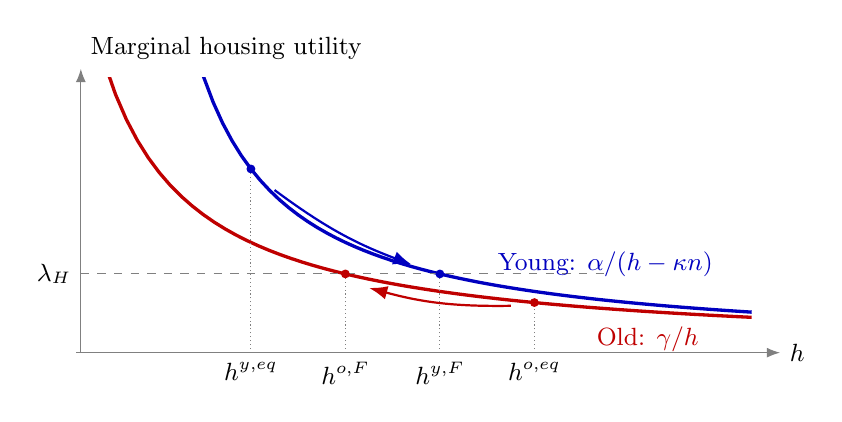
\begin{tikzpicture}[x=1.2cm,y=3.5cm,>=Latex, font=\small]
\draw[->,gray] (.65,0) -- (8.1,0) node[right,black] {$h$};
\draw[->,gray] (.7,0) -- (.7,1.03) node[above right,black] {Marginal housing utility};
\begin{scope}\clip (.71,.01) rectangle (8,1.0);
\draw[blue!75!black,very thick,domain=1.9:7.8,samples=60] plot(\x,{1/(\x-1)});
\draw[red!75!black,very thick,domain=.95:7.8,samples=60] plot(\x,{1/\x});
\end{scope}
\draw[gray,dashed] (.7,{2/7}) -- (6.3,{2/7});
\node[left] at (.7,{2/7}) {$\lambda_H$};
\draw[gray,densely dotted] (2.5,0)--(2.5,{2/3});
\draw[gray,densely dotted] (5.5,0)--(5.5,{2/11});
\draw[gray,densely dotted] (3.5,0)--(3.5,{2/7});
\draw[gray,densely dotted] (4.5,0)--(4.5,{2/7});
\fill[blue!75!black] (2.5,{2/3}) circle(1.6pt) (4.5,{2/7}) circle(1.6pt);
\fill[red!75!black] (5.5,{2/11}) circle(1.6pt) (3.5,{2/7}) circle(1.6pt);
\draw[->,blue!75!black,thick] (2.75,.59) to[bend right=8] (4.2,.32);
\draw[->,red!75!black,thick] (5.25,.17) to[bend left=8] (3.75,.235);
\node[blue!75!black,above] at (6.25,.24) {Young: $\alpha/(h-\kappa n)$};
\node[red!75!black,below] at (6.7,.13) {Old: $\gamma/h$};
\node[below] at (2.5,0) {$h^{y,eq}$};
\node[below] at (3.5,0) {$h^{o,F}$};
\node[below] at (4.5,0) {$h^{y,F}$};
\node[below] at (5.5,0) {$h^{o,eq}$};
\end{tikzpicture}
\end{center}
Matched owners with fixed fertility and slack size limits. At the planner's
allocation, the marginal utility of housing is equal across households.
\end{frame}

\begin{frame}{Fertility}
For a parent receiving a changed consumption--housing bundle,
\[
\dd n=\frac{\chi\,\dd c/x^2+\alpha\kappa\,\dd h/s^2}
{\vartheta/n^2+\chi^2/x^2+\alpha\kappa^2/s^2}.
\]
More space raises fertility if the accompanying loss of goods is small enough.
\medskip

If the planner chooses fertility jointly with consumption and housing,
\[
\bar c^{o,eq}\ge\bar x,\qquad
\bar h^{o,eq}\ge\frac\gamma\alpha\bar s,\qquad
h_R^{\max}>\bar h^{y,eq}
\quad\Longrightarrow\quad \bar n^J>\bar n,
\]
with at least one of the first two comparisons strict. These conditions
hold under the preceding income benchmark; planner caps may bind.
\medskip

Average private fertility after a fixed-fertility allocation need not rise.
The joint planner accounts for the adjustment of all resources together.
\end{frame}

\begin{frame}{Demographic transition}
\begin{center}
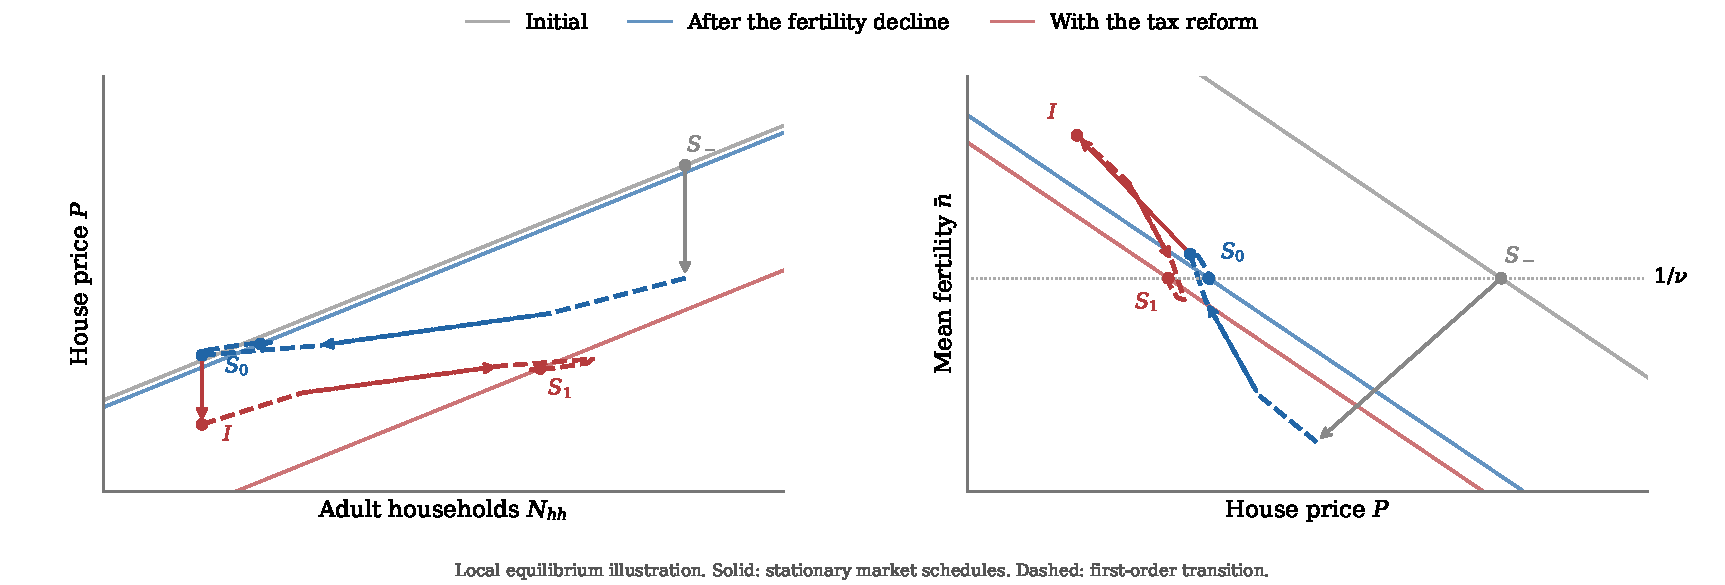
\includegraphics[width=.97\textwidth]{../../output/model/simplified_olg_amendments/consolidated_transition_figure.pdf}
\end{center}
\small
An exogenous fertility-taste decline starts the baseline transition.
A permanent rebated tax introduced at $I$ raises fertility on impact and
leads to $N_1>N_0$, under the note's local conditions.
Both terminal fertility rates equal $1/\nu$.
\end{frame}
\end{document}
